\documentclass[12pt, legalpaper]{article}
% 10pt es el tamaño de letra por default
% para modificarlo desde documentclass, solo permite 10pt, 11pt y 12. 
% Prueba comentario
\usepackage{graphicx} % Required for inserting images
\usepackage{float} % Se utiliza para el posicionamiento forzado de los elementos del documento (figuras y tablas)
\usepackage{subcaption} %mozaico de figuras
\usepackage{pdflscape}


\usepackage[table,xcdraw]{xcolor} %para añadir color a las celdas de una tabla
\usepackage[normalem]{ulem} %para subrayar texto
\useunder{\uline}{\ul}{}


\usepackage{enumitem} %generar listas con símbolos
\usepackage{pifont} %permite modificar los símbolos de las listas

\renewcommand{\labelitemii}{$ ? $} %para cambiar el símbolo por cuenta del usuario, este debe estar entre los sísmbolos de pesos. En este caso, se añade doble guión medio.
%labelitemi, al añadir otra "i" se indica el nivel de la tabla enumerada en el que se va a colocar el símbolo .

\usepackage{parskip} %para quitar sangría
\setlength{\parskip}{2mm}

\usepackage{blindtext} %texto aleatorio

\usepackage[spanish,mexico]{babel} %definimos el idioma español, para México.



\title{\Huge{Tiro con arco}}
\author{\small{Miguel Carrillo}}
\date{30 de Enero 2025}


\begin{document}

\maketitle

\begin{abstract}
    En este documento se explica en qué consiste el tiro con arco, se mencionan los accesorios necesarios para practicar este deporte y se detallan las reglas que rigen esta actividad.
\end{abstract}

\section{\LARGE{Introducción}}

Elaboración de mi \textbf{primer} \emph{documento} para visualizar las opciones del tipo de \texttt{documento}. 

El tiro con \huge{arco} es un deporte en el que los participantes disparan flechas usando un arco con el objetivo de alcanzar una diana o blanco lo más cerca posible del centro. La \large{precisión} es clave, y cada disparo es puntuado según la cercanía al centro de la diana. En la figura \ref{tiro1}, se muestra una foto de un competidor.

\begin{figure}[H]
    \centering
    %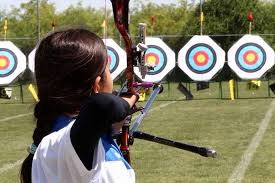
\includegraphics[scale=.5,angle=35]{tiro_arco.jpg} 
	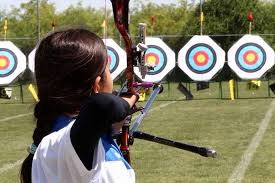
\includegraphics[scale=.5,angle=35]{tiro_arco.jpg}     
    \caption{Imagen ilustrativa del tiro con arco.}
    \label{tiro1}
\end{figure}

El tiro con arco es una práctica 'antigua' que comenzó como una técnica de caza y en la guerra. Sin embargo, como deporte organizado.
Corea del Sur domina este deporte a nivel olímpico. Han ganado más de 40 medallas (incluyendo alrededor de 27 de oro) desde que se reintrodujo en 1972. El éxito de Corea del Sur se atribuye a su sistema de entrenamiento riguroso y a la enorme popularidad del deporte en el país. 
%La probabilidad de que ganen los jefes de Kansas City es del 50\%.

\section{Mozaico de figuras}

A continuación se muestran los accesorios del tiro con arco. Por ejemplo, en la figura \ref{a} son las flechas y en la figura \ref{b} se observa la diana

\begin{figure}[H] % primeras dos subfiguras
    \begin{subfigure}{0.45\textwidth}
        \centering
        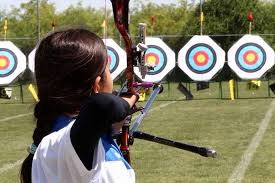
\includegraphics[scale=.35, angle=0]{tiro_arco.jpg} 
        \caption{Flechas}
        \label{a}
    \end{subfigure}
    \begin{subfigure}{0.45\textwidth}
        \centering
        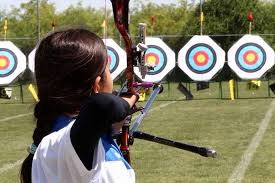
\includegraphics[scale=.35, angle=0]{tiro_arco.jpg}
        \caption{Soporte}
        \label{b}
    \end{subfigure} 
    
    \begin{subfigure}{0.45\textwidth} % otras dos subfigura
        \centering
        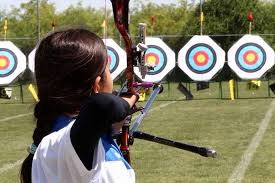
\includegraphics[scale=.35, angle=0]{tiro_arco.jpg}
        \caption{Visor}
        \label{c}
    \end{subfigure}
    \begin{subfigure}{0.45\textwidth}
        \centering
        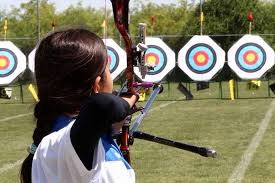
\includegraphics[scale=.35, angle=0]{tiro_arco.jpg}
        \caption{Arco}
        \label{c}
    \end{subfigure}
    \caption{Accesorios del tiro con arco.}
\end{figure}

\subsection{Más figuras}

\newpage

\begin{landscape}
    \begin{figure}[H]
        \centering
        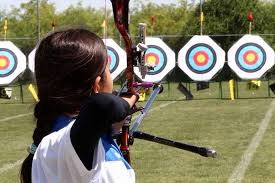
\includegraphics[scale=.35, angle=0]{tiro_arco.jpg}
        \caption{Figura más grande}
        \label{fig:enter-label}
    \end{figure}
\end{landscape}

\newpage

\section{Países ganadores en tiro con arco}

A continuación se muestra la tabla \ref{tab1} de ganadores de medalla de oro en tiro con arco desde 1900:

\begin{table}[H]
    \centering
    \begin{tabular}{|c|c|}
    \hline
      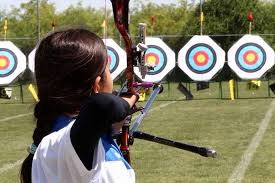
\includegraphics[scale=.35, angle=0]{tiro_arco.jpg}    &  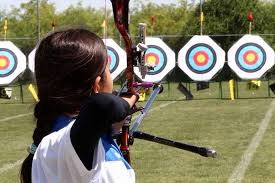
\includegraphics[scale=.35, angle=0]{tiro_arco.jpg}  \\
      \hline
      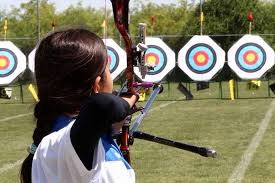
\includegraphics[scale=.35, angle=0]{tiro_arco.jpg}   & 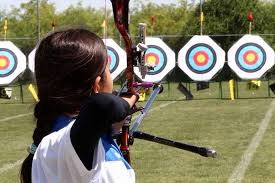
\includegraphics[scale=.35, angle=0]{tiro_arco.jpg}
    \end{tabular}
    \caption{Caption}
    \label{tab:my_label}
\end{table}





\begin{table}[H]
    \centering
    \begin{tabular}{c|c|c}
      Países   &  Cantidad de medallas & Part. en juegos olimp.\\
      México   &            10         & 20\\
      Corea del sur &       9          &  30\\
      China         &       8          & 10
    \end{tabular}
    \caption{Tabla histórica de medallas en tiro con arco.}
    \label{tab1}
\end{table}

%\noindent
Otra forma de generar o modificar la tabla 1 es con el generador de tablas en línea. De esta forma, podemos obtener la tabla \ref{tab2}


\begin{table}[H]
\begin{tabular}{|c|c|c|}
\hline
\rowcolor[HTML]{67FD9A} 
{\color[HTML]{333333} \textbf{Países}} & {\color[HTML]{333333} \textbf{Cantidad de medallas}} & {\color[HTML]{333333} \textbf{Participación en juegos olimpicos}} \\ \hline
\rowcolor[HTML]{FFFFFF} 
{\color[HTML]{333333} {\ul México}}           & {\color[HTML]{333333} 20} & {\color[HTML]{333333} {\ul 25}} \\ \hline
\rowcolor[HTML]{FFFFFF} 
{\color[HTML]{333333} \textit{Corea del Sur}} & {\color[HTML]{333333} 10} & {\color[HTML]{333333} 25}       \\ \hline
\rowcolor[HTML]{FFFFFF} 
China                                         & 5                         & 25                              \\ \hline
\end{tabular}
\caption{Nueva tabla.}
\label{tab2}
\end{table}



A continuación vamos a generar una lista no enumerada. Enlistemos los accesorios para practicar tiro con arco

\begin{itemize}  % representa el primer nivel de la lista no enumerada
    \item[\ding{36}] Flechas
        \begin{itemize} %segundo nivel de lista no enumerada
            \item[\ding{116}] Material 1
            \item Material 2
        \end{itemize}
    \item[\ding{61}] Arco
        \begin{itemize} %segundo nivel de lista no enumerado
            \item Compuesto
                \begin{itemize} %tercer nivel de lista no enumerada
                    \item Simple
                \end{itemize}
        \end{itemize}
    \item [\ding{61}]Soporte para flechas
    \item[\ding{61}] Pechera
    \item 
\end{itemize}

Aquí se muestra una lista enumerada.

\begin{enumerate}
    \item México
        \begin{enumerate}
            \item Categoría olímpica.
        \end{enumerate}
    \item China
    \item Corea del Sur
    \item Países Bajos
\end{enumerate}

\section{Reglas del tiro con arco}

\blindtext

\end{document}
